\documentclass{article}

\usepackage[final]{neurips_2023}
\usepackage[utf8]{inputenc} % allow utf-8 input
\usepackage[T1]{fontenc}    % use 8-bit T1 fonts
\usepackage{hyperref}       % hyperlinks
\usepackage{url}            % simple URL typesetting
\usepackage{booktabs}       % professional-quality tables
\usepackage{amsfonts}       % blackboard math symbols
\usepackage{nicefrac}       % compact symbols for 1/2, etc.
\usepackage{microtype}      % microtypography
\usepackage{xcolor}         % colors
\usepackage{float}
\usepackage{graphicx}

\title{Data Exploration Report 2025}

\author{% 
  Team TOOTHPASTE \AND
  Aral Cimcim (k11720457)
  \And
  Sandro Müller (k52010874)
  \And 
  Linus Madlener (k12310088)
  \And 
  Kevin Eberl (k12322451)
}

\begin{document}

\maketitle

\begin{contributions}
    \textcolor{gray}{
    Aral added the Case Study and investigated the Annotation Quality. (Task 1 + 2) \\
    Linus implemented the baseline for the Audio Features and analyzed the Text Features. (Task 3 + 4) \\
    Sandro and Kevin analyzed the Audio Features and experimented with different K-means/PCA parameters and metrics. (Task 3 + 4) \\
    }
  
  % \textcolor{gray}{E.g.: Tara Jadidi did the entire experimental setup, including the data-split and selection of features and pre-processing. Florian Schmid trained four different classifiers for the task, and Paul Primus was responsible for evaluating the classifiers, generating figures and writing the report.}
\end{contributions}

\section{Case Study}
Initially, we examined the distribution of annotators per file to characterize the annotation dataset. We found that the vast majority of files had been annotated by a single individual.

\begin{figure}[H]
    \centering
    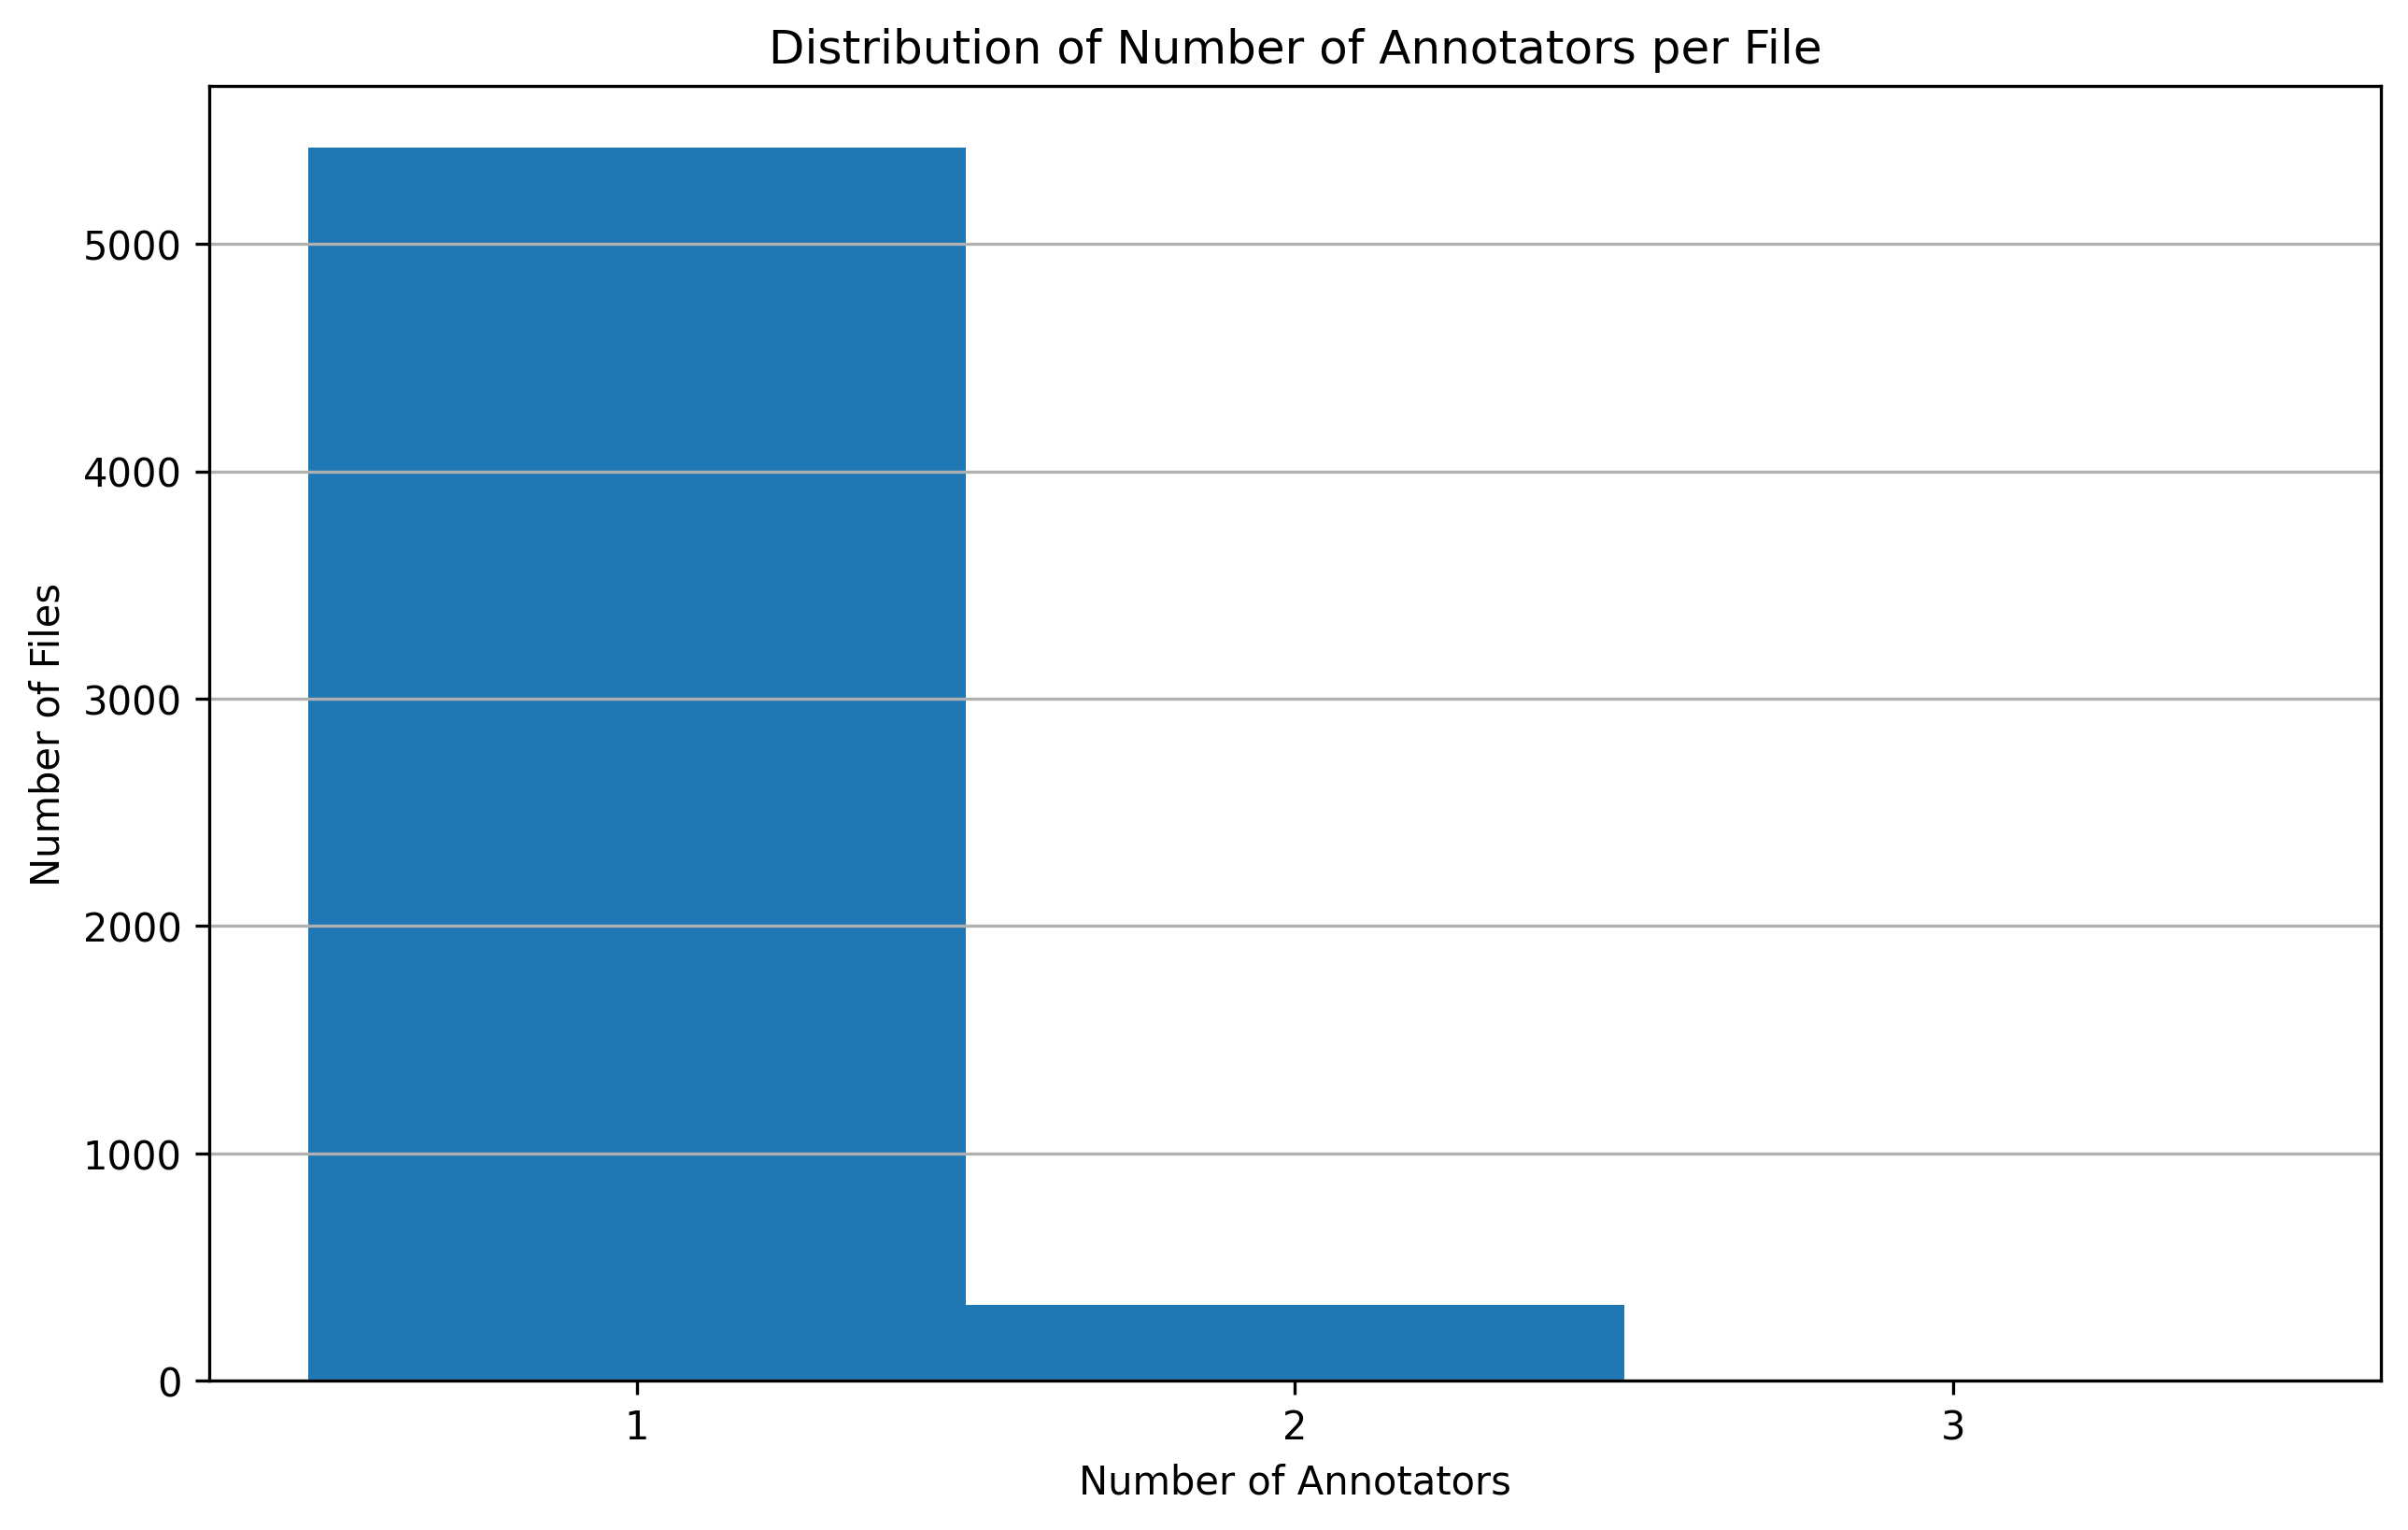
\includegraphics[width=0.5\linewidth]{annotators_per_file.png}
    \caption{Annotators per File}
    \label{fig:enter-label}
\end{figure}

For our case study, we then selected the following two files, both with two unique annotators:

\textbf{102744.mp3:}
This is a recording of several sentences that span around military content. The first annotator (ID starting with 114) has described it as "Military person speaking clearly and distinctly" while another annotator (ID starting with 946) has described it as "Calm mature male voice telling coordinates and military news", "Rough, a bit aggressive male voice repeating the same phrase 3 times". 

Annotator 114 did not separate the audio file into parts to consider the temporal characteristics fully while annotator 946 has divided the annotation into parts to emphasize repetitions in the recording. In terms of the textual annotations, annotator 946 has provided more detail in comparison to annotator 114 who seemed to have generalized the audio content. Both annotators have matching descriptions (946 has provided slightly more detail) when the metadata is taken into consideration; character, coordinates, latitude, longitude, mature, military, rough, screaming, yelling.

Overall, both annotators have followed the task description with varying granularity.

\vspace{3mm}

\textbf{110921.mp3:}
This is a recording of farmers collecting sheep from a field in Argentina by whistling and shouting. The first annotator (ID starting with 435 has described it as "dog barking", "farm animal sounds in the background", "a man whistles enthusiastically" while another annotator (ID starting with 611) has described it as "Persons shouting in a far outdoors", "Noise of sheep on a field outdoors". Both annotators have provided detailed information as per task description. The texts do match the metadata; argentina, del, forest, fuego, patagonia, rodeo, sheep, shout, tierra, whistle, whistling, blume, field-recording, felix. Both annotators have identified the main occurences in the recording such as "shouting", "field", "whistling" in a similar manner. 

The annotations do not deviate from the metadata content-wise.

\section{Annotation Quality}
\label{sec:headings}

For both files temporal annotations are relatively precise, the gaps are taken into consideration and separate events have been noted in accordance to the task description. It is worth mentioning that there is still a level of ambiguity in both files, which suggests subtle differences in the sound perception of human annotators.

The text annotations that correspond to the
same region are described similarly for the most part (e.g. annotator with ID 114 has not provided any gender for the person speaking in the recording, additionally the annotator did not reflect on the change of the speakers voice from calm to aggressive).

There is not a single number for the number of annotations per file in the whole dataset. Here we have listed the occurences of the top 10 annotations in \autoref{tab:annot}.

\begin{table}[H]
  \caption{Number of annotations per audio file (top 10)}
  \label{tab:annot}
  \centering
  \begin{tabular}{lr}
    \toprule
    filename & num. of annotations \\
    \midrule
    623187.mp3 & 96 \\
    94017.mp3  & 73 \\
    591203.mp3 & 65 \\
    518570.mp3 & 63 \\
    620967.mp3 & 42 \\
    406538.mp3 & 40 \\
    777608.mp3 & 40 \\
    352225.mp3 & 39 \\
    406166.mp3 & 38 \\
    272516.mp3 & 38 \\
    \bottomrule
  \end{tabular}
\end{table}

The shortest annotation consists of 2 characters while the longest contains 507 characters. Average annotation length (as characters) is 45 and (as words) is 7. There are 268243 words in total and 10476 unique words resulting in a vocabulary diversity ratio of 0.004.
There are 2684 misspelled words and a typo frequency rate of 0.01 as the typo count over the whole vocabulary. (We have not used additional tables for the annotation quality task as they would extend the number of pages)

There are a few poor quality annotations in the data set such as "man laughs", "dog barking", "A foot step", "click". A method to solve this issue could be to set a minimum and maximum length for the annotations and filter them from the data set.

\section{Audio Features}
To assess the relevance of our audio features, we first standardized all feature vectors. For each annotated segment and silent interval, we then computed a fixed-length representation by averaging each feature over time within that region. This gives us a concise vector per region, suitable for clustering and visualization.

\begin{figure}[H]
    \centering
    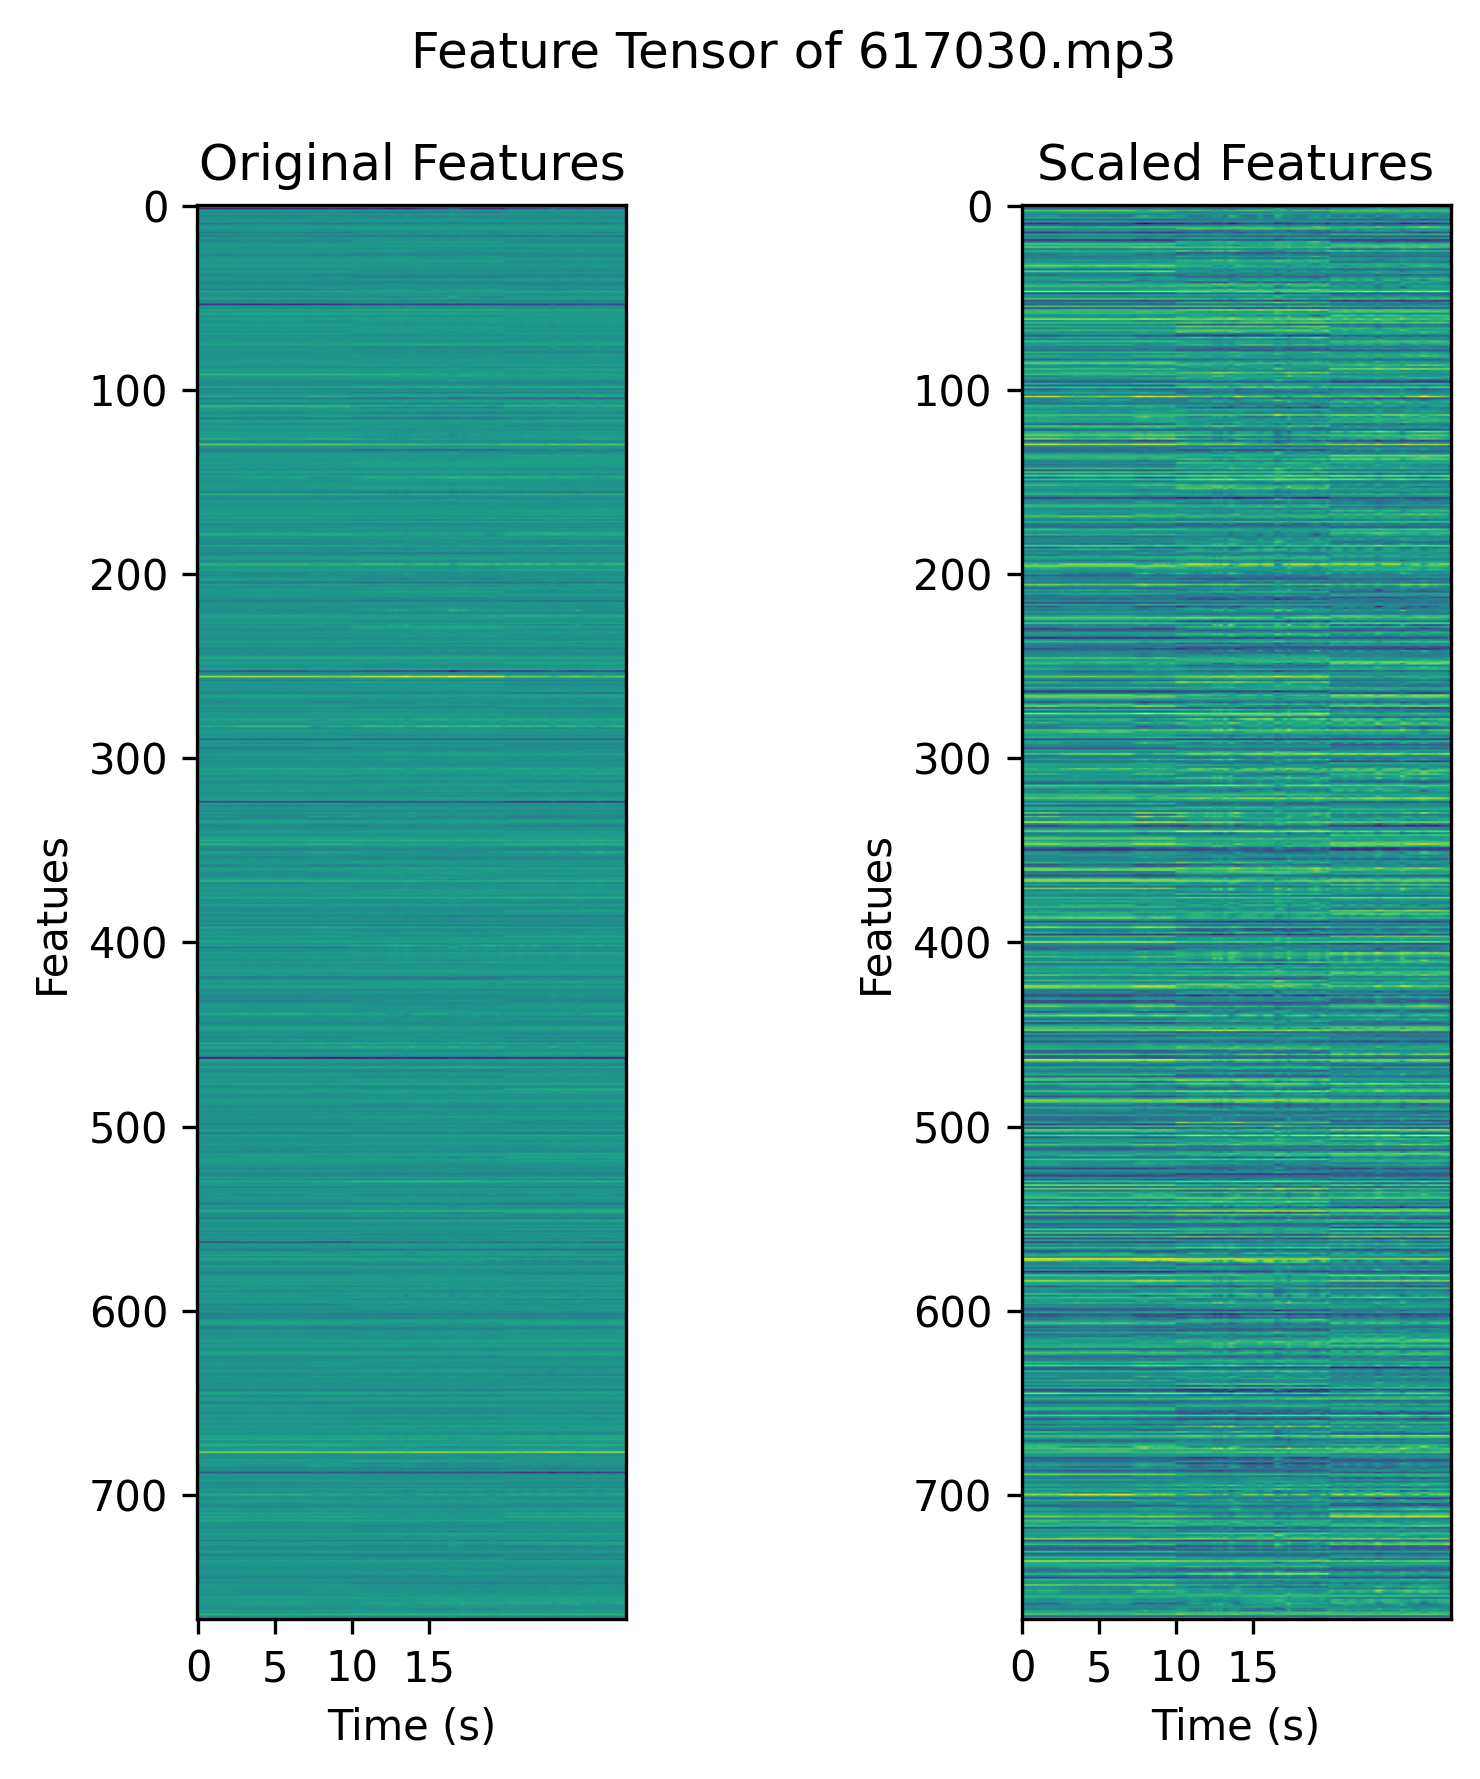
\includegraphics[width=0.25\linewidth]{feature_tensor.png}
    \caption{Example Feature Tensor}
    \label{fig:feature_tensor}
\end{figure}

We tried to find meaningful clusters (k) using different quality metrics (\autoref{tab:quality_metrics}):
\begin{table}[H]
  \centering
  \caption{Quality Metrics (k = 25)}
  \label{tab:quality_metrics}
  \begin{tabular}{@{} l c c c @{}} 
    \toprule
    Metric & Score & Formula & Ideal \\
    \midrule
    Silhouette Score & 0.089 & $s = \frac{1}{N}\sum_{i=1}^N \frac{b_i - a_i}{\max(a_i,b_i)}$ & $\uparrow$ higher \\
    Calinski-Harabasz Index & 936.9 & $\mathrm{CH} = \frac{\mathrm{tr}(B_k) \backslash (k - 1)}{\mathrm{tr}(W_k) \backslash (N - k)}$ & $\uparrow$ higher \\
    Davies-Bouldin Index & 2.697 & $\mathrm{DB} = \frac{1}{k}\sum_{i=1}^k \max_{j\neq i} \frac{\sigma_i + \sigma_j}{d(c_i,c_j)}$ & $\downarrow$ lower \\
    \bottomrule
  \end{tabular}
\end{table}

Applying K-means clustering with k = 25 to these region vectors revealed that silent intervals do not consolidate into a single cluster; instead, they are dispersed across many clusters. 

A complementary t-SNE visualization (\autoref{fig:tsne_silent}) confirms substantial overlap between silent and annotated regions, indicating that silent regions do not form distinct cluster in the full feature space.

\begin{figure}[H]
    \centering
    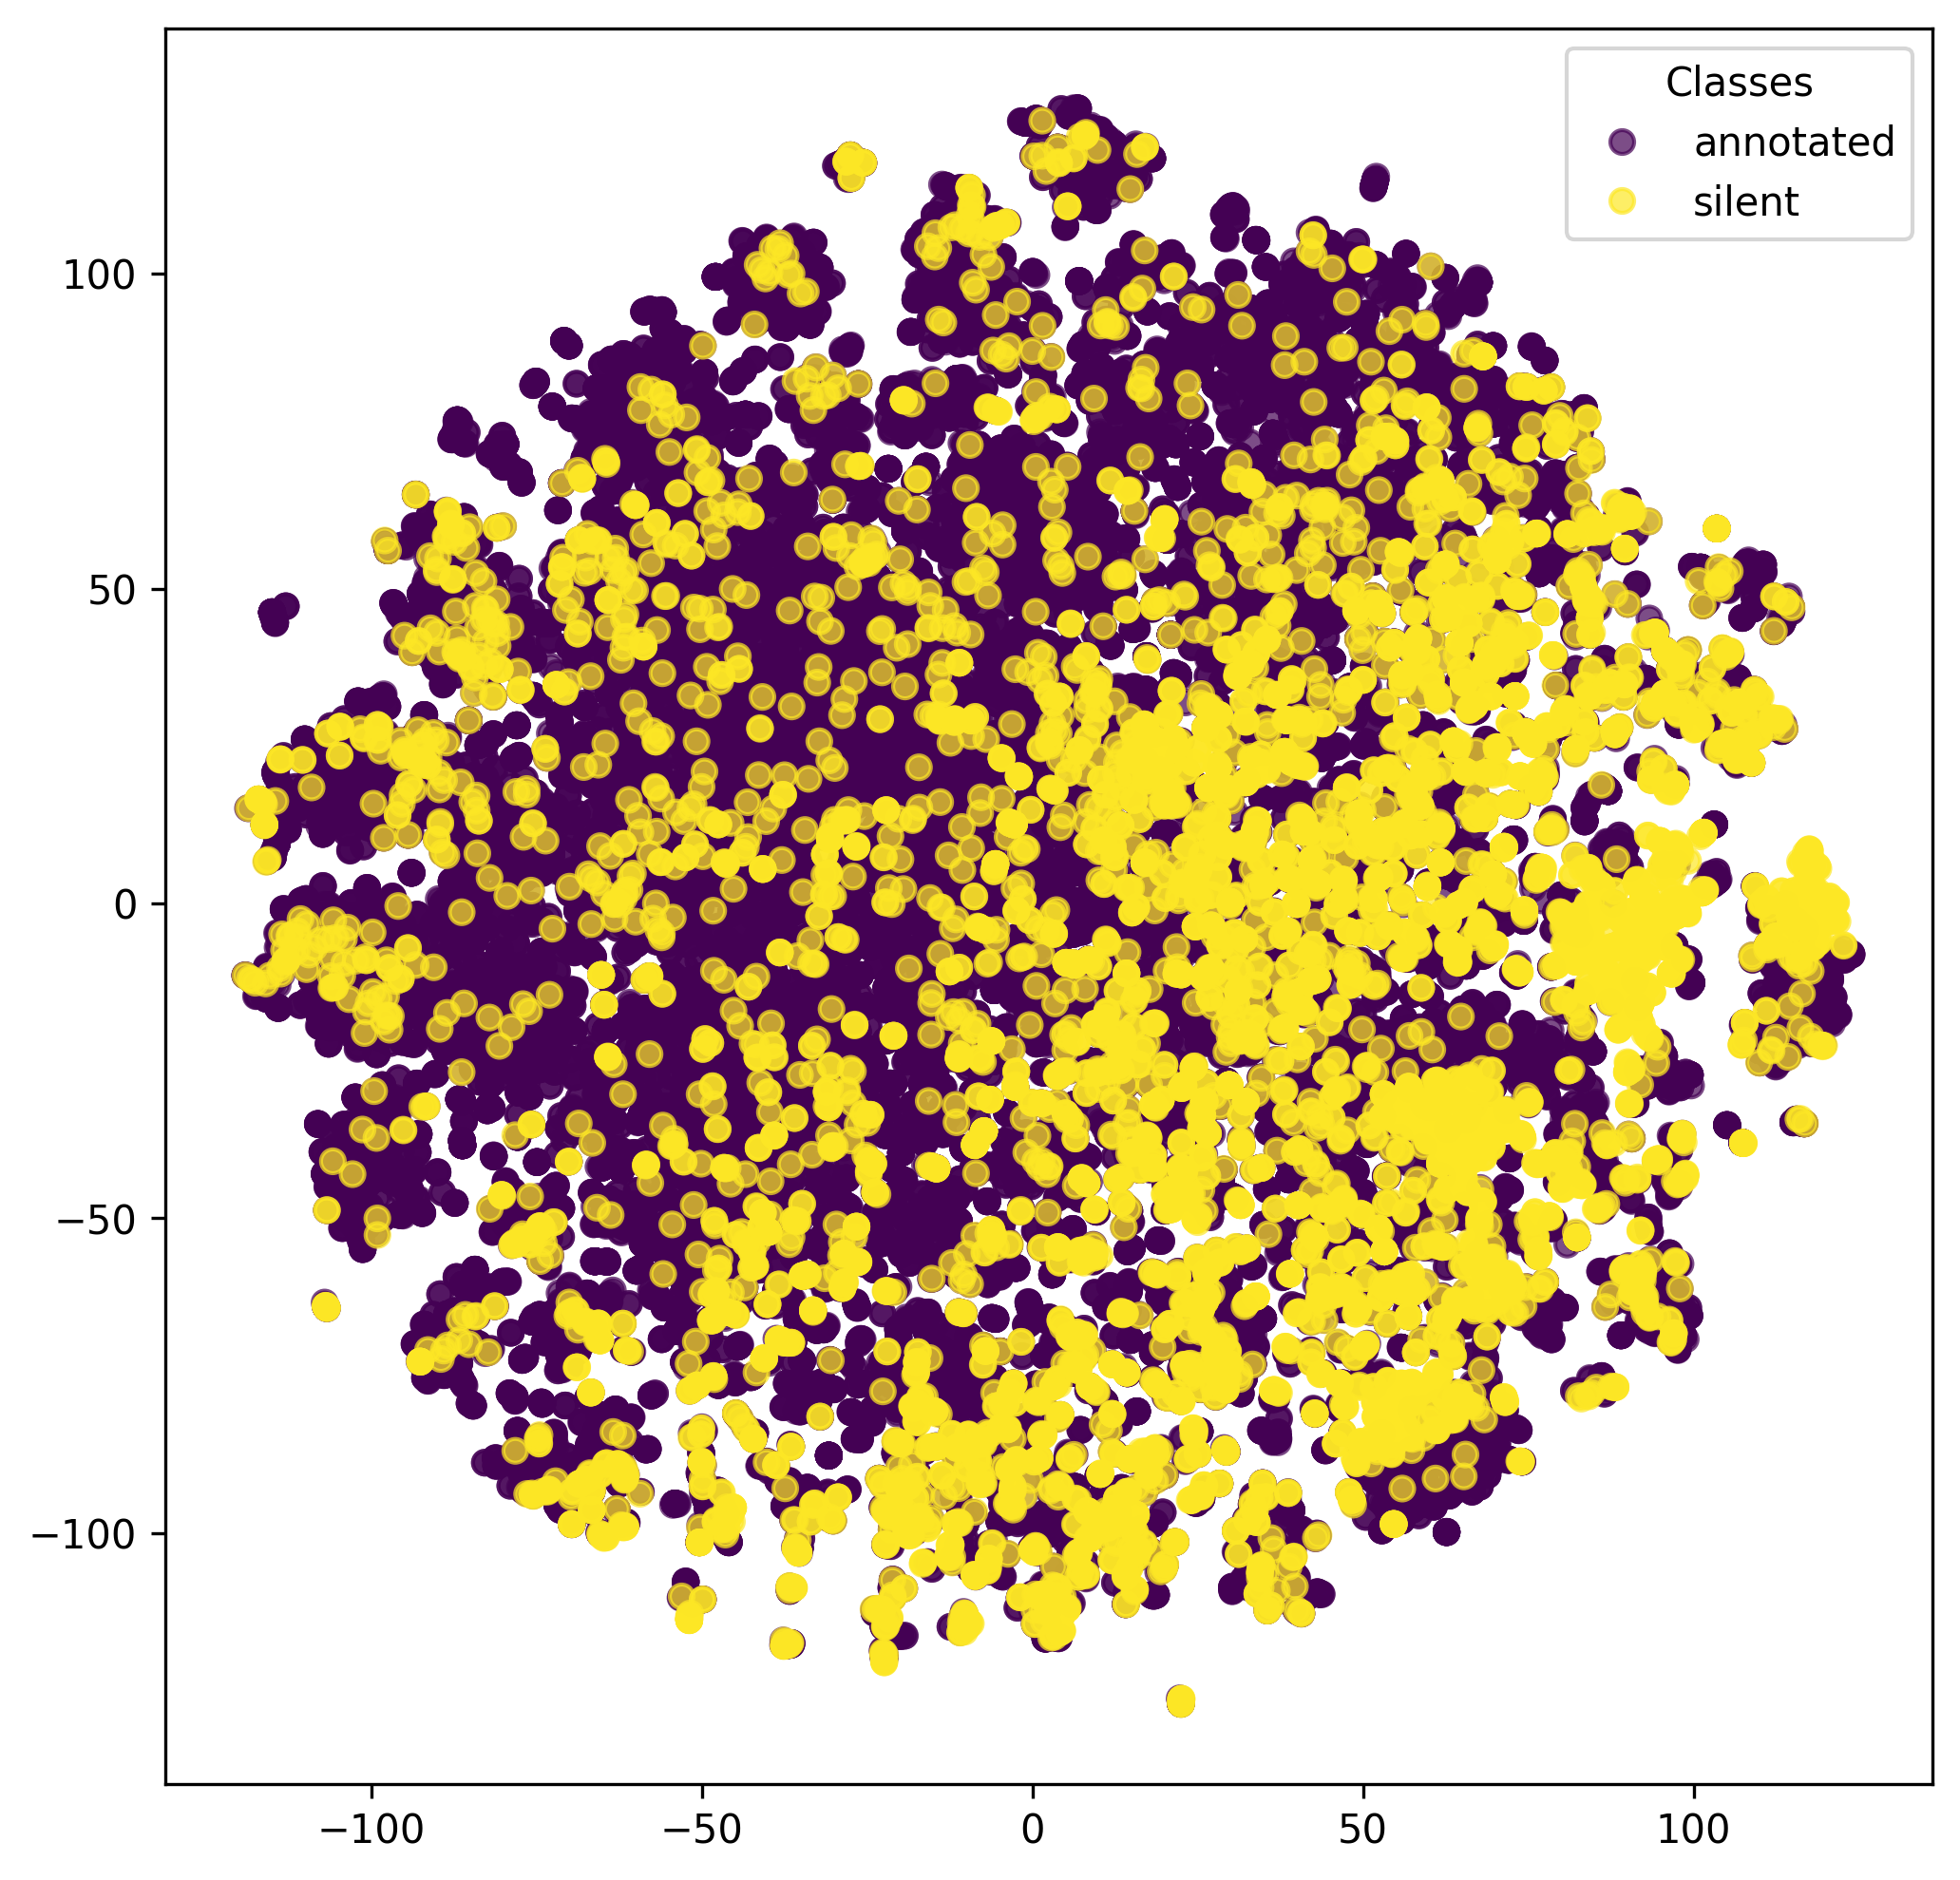
\includegraphics[width=0.4\linewidth]{tsne_silent.png}
    \caption{t-SNE Classes}
    \label{fig:tsne_silent}
\end{figure}

\section{Text Features}
We performed an analogous analysis on the textual annotations. \\
Using K-means (k = 25) followed by t-SNE for visualization (\autoref{fig:textual_clusters}), we identified several coherent clusters of annotation text.

\begin{figure}[H]
    \centering
    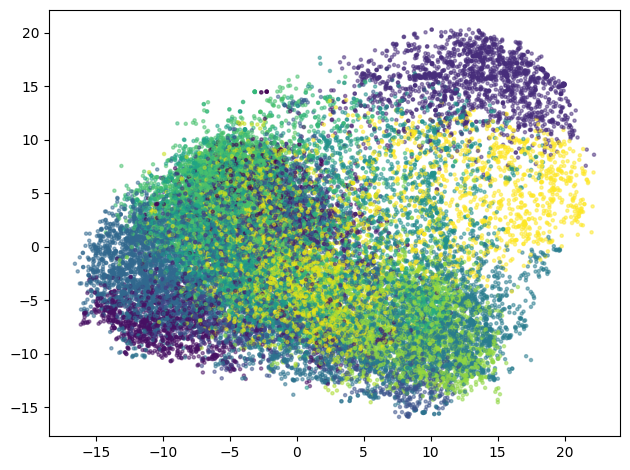
\includegraphics[width=0.5\linewidth]{textual_clusters.png}
    \caption{Textual Clusters (t-SNE)}
    \label{fig:textual_clusters}
\end{figure}

\subsection{Clustering: Dog sounds}
We designed a labeling function to find the textual annotations related to dog sounds and tried to find a meaningful cluster:

\begin{figure}[H]
    \centering
    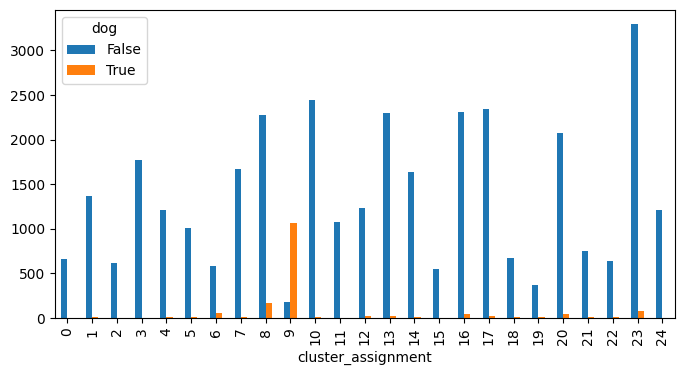
\includegraphics[width=0.5\linewidth]{dog_clusters.png}
    \caption{Clustering: dog}
    \label{fig:dog_clusters}
\end{figure}

When we take a closer look at the annotations in cluster 9 - which seems to predominantly include dog sounds - there are indeed many occurrences which indicate the specific sound source. (see \autoref{tab:dog_annot})

\begin{table}[H]
  \caption{Cluster 9 annotations}
  \label{tab:dog_annot}
  \centering
  \begin{tabular}{lr}
    \toprule
    idx & annotation \\
    \midrule
    12 & A dog is barking furiously.  \\
    53 & Dog barking loudly in the background \\
    58 & A noise humming constantly. \\
    62 & A dog barking \\
    93 & a single dog bark \\
    94 & A dog growls \\
    104 & pigs growling loudly and aggressively. \\
    110 & dog barking \\
    129 & Dog barking husky \\
    211 & Very loud dog bark \\
    \bottomrule
  \end{tabular}
\end{table}

\subsection{Clustering: Cat sounds}
As we did previously with dog sounds, we also wanted to identify a cluster consisting of cat sounds:

\begin{figure}[H]
    \centering
    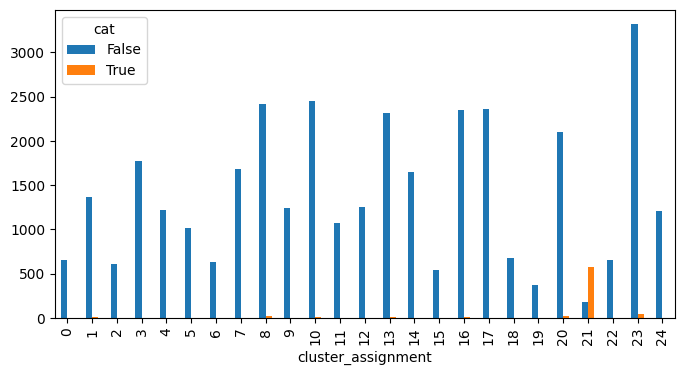
\includegraphics[width=0.5\linewidth]{cat_clusters.png}
    \caption{Clustering: cat}
    \label{fig:cat_clusters}
\end{figure}

This time we look at cluster 21 - which should consist mostly of cat sounds - to analyze the text annotations. (see \autoref{tab:cat_annot})

\begin{table}[H]
  \caption{Cluster 21 annotations}
  \label{tab:cat_annot}
  \centering
  \begin{tabular}{lr}
    \toprule
    idx & annotation \\
    \midrule
    3 & A high pitch meowing coming from a cat \\
    27 & Continuous purrr like sound which resembles to... \\
    63 & opening or closing a zip noise in background, ... \\
    107 & Low-pitched cat meow with low background noise. \\
    123 & A ball kicking the ground one time, distantly. \\
    147 & very weak meow of a cat \\
    160 & small cat is worried meowing \\
    164 & Cat meowing \\
    165 & a cat growl multiple times \\
    184 & A cat miaus briefly and loudly indoors. \\
    \bottomrule
  \end{tabular}
\end{table}

Again, there are some outliers, but the vast majority of annotations specify a cat as the sound source.

\section{Conclusion}
Because our dataset contains many unique sound events and most files were labeled by a single annotator, it inevitably reflects individual biases. However, clustering the textual annotations successfully revealed groups that correspond to specific semantic labels.

\end{document}